\section{Funcionamento}

Como apresentado na subseção \ref{sec:definicoes}, as DTNs dependem das oportunidades de contato para a retransmissão de mensagens. Por sua vez, os contatos são influenciados diretamente pelo intervalo de busca por dispositivos próximos, visto que durante um período de espera um nó pode acabar não contatando outros que estava próximos. A partir daí, o gerenciamento do intervalo de busca de acordo com a probabilidade de contato numa determinada localização permite o ajusto dinâmico do intervalo fixo de espera de 32 segundos proposto por \cite{denis_artigo}.

O comportamento praticamente estocástico dos dispositivos, como os das moléculas de sacarose dissolvendo-se em água, torna a previsibilidade da localização dos contatos dificultosa em diversos cenários, como o das Redes Móveis Ad Hoc e o ZebraNet. Todavia, a concentração pode ser calculada por meio de um mapeamento dinâmico utilizando módulos de GPS dos dispositivos.

\subsection{O Mapeamento Dinâmico}

Inicialmente, uma divisão do mapa em regiões de igual tamanho é realizada. A partir daí, ao estabelecerem contato, os dispositivos envolvidos registram este em uma \emph{Tabela de Mapeamento de Regiões} (TMR). É por meio dessa tabela que cada nó tem uma visão global do mapa, pois sempre armazenam as quantidades de contatos registrados em cada uma das regiões pelas quais cada nó passou. Ao registrar um contato, é feita uma consulta GPS para determinar com precisão em que região o nó se encontra e contabilizar esse evento.

Após o registro do contato na tabela, os nós trocam suas TMRs para dinamizar o mapeamento e permitir que tenham acesso a dados de regiões pelas quais eles ainda não passaram. É passível de afirmação que o compartilhamento das TMRs implementa a prosa descrita na subseção \ref{subsec:gradientes_desafios}, onde dois nós, educadamente, compartilham um com o outro as informações que possuem acerca das regiões por onde passaram.

É de grande importância o estudo quanto a forma de mesclagem das tabelas de mapeamento. Durante o desenvolvimento deste trabalho foram consideradas três formas para tal, sendo elas:

\begin{itemize}
    \item \textbf{Mesclagem por Soma:} Nesta modalidade de mesclagem, para cada registro do nó contatado, se o dispositivo que recebeu a tabela, já possui alguma informação do registro é realizada uma soma dos valores. Caso contrário, o valor é adicionado a um novo registro na tabela. Em suma esta estratégia parece interessante, mas, durante as simulações, foi percebido que o comportamento cíclico de alguns nós causa a geração de registros extremamente discrepantes com relação ao comportamento real da rede, além de, após longos períodos de simulação, ocorrerem problemas com \emph{overflow} de variáveis mesmo quando utilizando \emph{64bits} de tamanho;
    \item \textbf{Mesclagem Incremental:} Ao realizar a mesclagem das tabelas, para cada registro do nó contatado, se o dispositivo já possui algum registro daquela região, é feito um incremento de um no registro local. Caso contrário, o valor é copiado para um novo registro na tabela. Esta abordagem não se mostrou satisfatória durante as simulações pois não conseguiu representar de forma satisfatória o comportamento real do mapa de regiões, ocorrendo momentos em que os valores ficaram totalmente incoerentes com a realidade;
    \item \textbf{Mesclagem por Substituição do Maior:} Nesta forma de mesclagem, para cada registro do outro nó, caso já exista um registro na tabela local e este seja menor que o do outro nó, é realizada a substituição. Caso não exista registro local, o valor é copiado. Caso contrário, ou seja, o valor local é maior que o do outro dispositivo, nada é feito. Esta forma de mesclagem foi a que melhor conseguiu representar o mapa regiões real, apresentando proporções coerentes com o comportamento real da rede.
\end{itemize}

Neste trabalho é considerada a mesclagem por meio da substituição do maior elemento devido ao fato de ter apresentado, durante as simulações, melhor representação do comportamento real da rede num ambiente onde o mapa é construído de forma independente e dinâmica.

Dados dois nós \emph{A} e \emph{B} localizados próximos e com o nó \emph{A} realizando buscas, o comportamento do mapeamento dinâmico é descrito pela Figura \ref{mapeamento}. É importante ressaltar que, neste trabalho, não foi considerada a sobrecarga gerada pela troca das TMRs.

\begin{figure}[htp!]
\centering
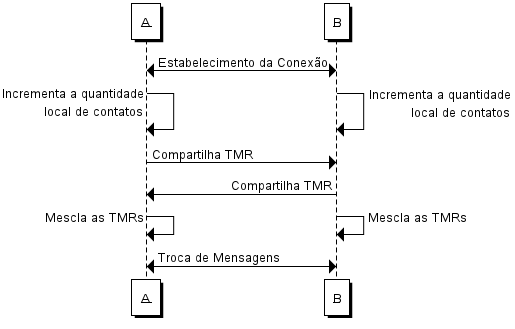
\includegraphics[width=0.75\textwidth]{figuras/cap_4/mapeamento.png}
\caption{Diagrama de Sequência do Mapeamento Dinâmico utilizando as TMRs}
\label{mapeamento}
\end{figure}

\subsection{Dinamização do Intervalo de Busca}
\label{sec:dinamizacao_intervalo_busca}
Tendo as Tabelas de Mapeamento de Regiões construídas dinamicamente, os dispositivos podem calcular livremente a probabilidade de contato em cada uma das regiões definidas previamente. Como pode ser visto em \cite{hazzan2013fundamentos}, a probabilidade de um evento $A$ ocorrer ($P(A)$), pode ser descrita por:

\begin{equation}
P(A)=\frac{n(A)}{n(\Omega)}
\end{equation}

Onde $n(A)$ é a quantidade de casos favoráveis a $A$ e $n(\Omega)$ é o número de resultados do experimento.

Tendo noção da probabilidade de contato $P(r)$ de um nó encontrar outro na região $r$, há duas decisões que um nó pode tomar: Aumentar ou diminuir o intervalo de buscas. Se um nó está em uma região com alta probabilidade de contato, este pode gastar mais a sua bateria visando aproveitar melhor as oportunidades daquela região. Caso a probabilidade seja muito pequena, o nó possui menor chance de tirar proveito de sua bateria, fazendo mais sentido economizá-la para um momento mais oportuno.

Observa-se então que, a concentração estimada em uma determinada região é, na verdade, a probabilidade de contato nessa localidade. A justificativa para isto baseia-se na grande importância dos contatos para as DTNs e na limitada visão que os dispositivos possuem quanto a quantidade de dispositivos próximos, visto hardware limitado que geralmente possuem. Além disso, regiões com altas taxas de contatos tendem a ser mais frequentadas por muitos dispositivos, influenciando diretamente na concentração efetiva da localidade.

Existe, entre a concentração, ou probabilidade de contado, e o intervalo de busca, um relacionamento de proporcionalidade inversa, ou seja, quanto maior a probabilidade, menor o intervalo de busca, e, quanto menor a probabilidade, maior o intervalo de busca. Sendo assim, é preciso descrever este relacionamento por meio de uma equação que o representa corretamente.

A proposta deste trabalho é que, dado um intervalo mínimo de busca $Im$, um intervalo máximo $IM$ pré-definidos e a probabilidade de contato na região em que o nó se encontra $P(r)$, pode-se descrever o intervalo de busca dito ideal $Ir$ como:

\begin{equation}
Ir=Im + (1-P(r))(IM-Im)
\label{eq_intervalo_ideal}
\end{equation}

O relacionamento de proporcionalidade inversa é descrito pelo termo $1-P(r)$, este pode ainda ser entendido como a probabilidade do contato não ocorrer \cite{hazzan2013fundamentos}. O termo $IM-Im$, quando multiplicado por $1-P(r)$ e posteriormente somado a $Im$, garante queo intervalo $Ir$ seja no máximo igual a $IM$  e no mínimo igual a $Im$.

O intervalo de busca ideal da região atual de um determinado nó da rede é calculado sempre quando este inicia um novo ciclo de busca que, por sua vez, nada mais é do que um período de procura por nós seguido de um intervalo de espera $Ir$ da região $r$ onde ele se encontra.

Quando a rede inicia sua operação, é notável que, durante certo período de tempo, os nós não possuem dados em suas TMRs ou estes ainda não são fieis ao comportamento estimado da rede. Para contornar este problema, foi proposto que a técnica passasse por um período de aquecimento, ou \emph{warmup time}, que é um período pré-definido onde os nós não fazem uso de suas TMRs e definem seus intervalos de busca como sendo o intervalo ideal de 32 segundos proposto por \cite{denis_artigo}.

Ainda existe o caso onde um determinado nó pode não ter dados sobre os contatos registrados na região onde ele se encontra. Para este caso, foi considerado o intervalo de busca de 32 segundos.

O diagrama da Figura \ref{diagrama} descreve de forma sucinta o funcionamento da técnica quanto a dinamização do intervalo entre as buscas por dispositivos.

\begin{figure}[htp!]
\centering
\includegraphics[width=0.75\textwidth]{figuras/cap_4/diagrama.png}
\caption{Diagrama de fluxo da dinamização do intervalo de busca}
\label{diagrama}
\end{figure}